%%%%%%%%%%%%%%%%%%%%%%%%%%%%%%%%%%%%%%%%%%%%%%%%%%%%%%%%%%%%%%%%%%%%%%%%%%%%%%%%%%%%%%%%%%%%%%%%%%%%%%%%%%%%%%%%%%%%%%%%

%%%%%%%%%%%%%%%%%%%%%%%%%%%%%%%%%%%%%%%%%%%%%
\chapter[Modeling interdependent infrastructure system reliability using `Muir webs']{Modeling interdependent infrastructure system reliability using `Muir webs' \footnote[10]{This work was published as a paper entitled ``Broadening the discourse on infrastructure interdependence by modeling the `ecology' of infrastructure systems'' in \emph{Applications of Statistics and Probability in Civil Engineering} \cite{LaRocca2011b}. This paper won first place in the Chesapeake Water Environment Association Student Paper Competition in 2011. I also won the Society for Risk Analysis Engineering and Infrastructure Specialty Group Student Merit Competition in 2011 for this work.}}
\label{ch4}
%%%%%%%%%%%%%%%%%%%%%%%%%%%%%%%%%%%%%%%%%%%%%

%%%%%%%%%%%%%%%%%%%%%%%%%%%%%%%%%%%%%%%%%%%%%%%%%%%%%%%%%%%%%%%%%%%%%%%%%%%%%%%%%%%%%%%%%%

%%%%%%%%%%%%%%%%%%%%%%%%%%%%%%%%%%%%%%%%%%%%%
\section{Introduction}
\label{sec:ch4:intro}
%%%%%%%%%%%%%%%%%%%%%%%%%%%%%%%%%%%%%%%%%%%%%

As discussed in previous sections, the large geographic scale of infrastructure systems and the inherent complexities of the interactions among infrastructure systems within the natural and anthropogenic environments in which they exist pose significant challenges for modeling the performance and reliability of interdependent infrastructure systems. Standard methods developed in civil engineering for use with single structural systems do not extend well to large-scale infrastructure systems. In this chapter, I investigate the possibility of using methods used to model another set of large-scale, complex, adaptive networked systems - ecological networks - to model the performance and reliability of interdependent infrastructure systems. I show that a particular model construction, that of a Muir web from Sanderson (2009)\cite{Sanderson2009}, provides an approach for more accurately capturing and modeling the complex interactions inherent in infrastructure systems, substantially expanding the influences that can be considered in infrastructure performance and reliability analysis beyond the relatively simple interactions considered with traditional approaches.

Civil engineers have developed a strong set of tools for analyzing the probability of failure of a structural component or structural system given an external load. The traditional approach to this problem is to use a fragility curve-based approach. A fragility curve gives the probability of the structural component or system being in each of the possible end damage states as a function of the measure of the hazard loading. These curves are often developed based on structural reliability methods, observed data, or a combination of the two. This approach is in widespread use and forms the basis of the infrastructure risk assessment approaches in HAZUS, the World Bank's CAPRA method, the MAEVis approach from the Mid-America Earthquake Center, and the matrix-based approach of Kang (2008)\cite{Kang2008}. Fragility curves have been developed for aspects of infrastructure systems such as power poles and water pipes for a number of hazards including earthquakes and hurricanes.

Two critical limitations of traditional fragility-based approaches are: (1) they generally assume that failure probabilities can be accurately represented as depending on a single measure of hazard loading and (2) they assume that failures of infrastructure components are conditionally independent given the hazard loading measure. While it is possible to develop a multi-dimensional fragility curve, \emph{i.e.}, one in which the failure probability depends on multiple dimensions of the hazard event, this is rarely done. Instead, the probability of failure is modeled as depending on a single dimension of the hazard situation. For example, in earthquake infrastructure risk assessment, fragility curves represent the failure probability as depending on a single measure of ground motion such as peak ground acceleration or peak spectral acceleration \cite{Cagnan2005}. Similarly, for power system risk assessment for hurricanes, traditional fragility-based approaches give the probability of failure as a function of wind speeds measures (\emph{e.g.}, maximum three second gust) alone (\emph{e.g.}, Booker \emph{et al.} (2010)\cite{Booker2010}, Han \emph{et al.} (2008)\cite{Han2008}, and Winkler \emph{et al.} (2010)\cite{Winkler2010}). However, this single demand parameter dependence is not accurate for some hazards. For example, Liu \emph{et al.} (2005)\cite{Liu2005}, Han \emph{et al.} (2009)\cite{Han2009b}, and Guikema \emph{et al.} (2010)\cite{Guikema2010} have shown that for hurricanes, there are many additional factors that are important in determining damage beyond gust wind speed, that these factors are not particularly well-correlated with wind speed, and that wind speed measures are not even the most important of the considered factors. Fragility-based approaches based on single demand parameters cannot yield an accurate estimate of system performance and reliability in such situations. 

%%%%%%%%%%%%%%%%%%%%%%%%%%%%%%%%%%%%%%%%%%%%%%%%%%%%%%%%%%%%%%%%%%%%%%%%%%%%%%%%%%%%%%%%%%

%%%%%%%%%%%%%%%%%%%%%%%%%%%%%%%%%%%%%%%%%%%%%
\section{Ecological networks and Muir webs}
\label{sec:ch4:muirwebs}
%%%%%%%%%%%%%%%%%%%%%%%%%%%%%%%%%%%%%%%%%%%%%

Ecological networks share many similarities with infrastructure networks. They are large-scale, involve complex interactions among many sub-networks, and exhibit failures in the face of external loading events. A number of different modeling approaches have been developed for estimating the `performance' (\emph{e.g.}, the integrity, productivity) of ecological networks (\emph{e.g.}, MacArthur (1955)\cite{MacArthur1955}, Lindeman (1942)\cite{Lindeman1942}, Elton (1927)\cite{Elton1927}, Winberg(1972)\cite{Winberg1972}). Traditional approaches rely on the concept of a food web \cite{Paine1980}. The inputs and outputs of the different subnetworks are modeled, and the growth and death of populations of organisms are estimated based on inputs (food consumed) and outputs (deaths) \cite{Pahl-Wostl1993}.  This is akin to an input-output based approach for modeling infrastructure network performance (\emph{e.g.}, Haimes \emph{et al.} (2005)\cite{Haimes2005}), and, like fragility-based approaches for infrastructure risk assessment, a food web significantly simplifies the representation of ecological network performance. A food web assumes that food is the limiting factor in the growth of a population, ignoring the host of other factors that are known to influence the presence, size, and spatial extent of a population \cite{Smith1972}. Sanderson (2009) \cite{Sanderson2009} proposed a Muir web as a way of substantially extending the sets of driving factors and relationships considered in modeling the performance of a set of ecological networks.

A Muir web represents not only the predator-prey relationships considered in traditional food webs; it also considers the dependence of populations on environmental factors. Originally developed for reconstructing the natural history of Manahatta (pre-colonization Manhattan Island), Muir webs include factors such as topography, the spatial and temporal distribution of disturbance, water, wetlands, soil types, wind and rainfall.  These factors are known to affect the spatial distribution of plant and animal species. These factors are then represented in the form of a graph. Nodes are the species (\emph{e.g.}, beaver) and factors (\emph{e.g.}, fire-induced forest clearings or wetlands). The edges in the graph represent dependencies. For example, for a beaver to be present, it needs to have appropriate types of trees and access to a ``slowly meandering'' stream. The next higher levels of edges represent the dependencies of each of the things the beaver depends on. For example, some types of trees needed depend on open woods, and proper soil types, light exposure, and soil moisture levels. By examining each species of the ecological system systematically, the full set of dependencies is captured, substantially expanding the relationships considered beyond the traditional predator-prey relationships included in food webs.

In this work I propose applying the concept of a Muir web to infrastructure systems. Each element of the infrastructure system is examined, and its dependencies are noted. For example, a pump in a water distribution system needs electric power, a stable foundation, an operator, water input, a pipe connection to output to, and maintenance. 

%%%%%%%%%%%%%%%%%%%%%%%%%%%%%%%%%%%%%%%%%%%%%%%%%%%%%%%%%%%%%%%%%%%%%%%%%%%%%%%%%%%%%%%%%%

%%%%%%%%%%%%%%%%%%%%%%%%%%%%%%%%%%%%%%%%%%%%%
\section{Example}
\label{sec:ch4:example}
%%%%%%%%%%%%%%%%%%%%%%%%%%%%%%%%%%%%%%%%%%%%%

To demonstrate the application of the Muir web approach to infrastructure systems, I conducted a simple case study using a fictitious system including water distribution, power distribution, and transportation (Figure \ref{fig:ch4:infrastructures}).  The networks for each of these consist of elements commonly present in such systems: the water system is comprised of a lake, treatment plant, tank, chlorine booster, valve, pump, and pipes; the power system contains a generation station, substation, switch, lines, and poles; and the transportation system includes roads.  The performance of each element is dependent on other elements in the system as well as additional factors, such as soil type (\emph{e.g.}, for poles and buildings), presence of operators (\emph{e.g.}, for treatment plant and generation station), and maintenance (for all elements).  The Muir web describing the relationship between system elements and outside factors is presented below in Figure \ref{fig:ch4:muirweb}.

%--------------------------------------------
% TABLE -------------------------------------

\begin{table}
\centering
\begin{tabular}{l l}
\toprule
\bf{System element} & \bf{P(failure)}\\
\midrule
Lake&0.0\\
Treatment plant&\\
\hspace{10pt}Buildings&$N(90,35)$\\
Tank&\\
\hspace{10pt}Foundation, soil 1 & $N(120,30)$\\
\hspace{10pt}Foundation, soil 2 & $N(160,50)$\\
Chlorine booster&\\
\hspace{10pt}Shelter & $N(90,35)$\\
\hspace{10pt}Foundation & $N(90,35)$\\
Valve&\\
\hspace{10pt}Components & 0.0\\
Pump&\\
\hspace{10pt}Shelter & $N(90,35)$\\
\hspace{10pt}Foundation & $N(90,35)$\\
Pipe&\\
\hspace{10pt}Components & $N(130,45)$\\
Generation station&\\
\hspace{10pt}Components & $N(200,60)$\\
Substation&\\
\hspace{10pt}Foundation, soil 1 & 0.05\\
\hspace{10pt}Foundation, soil 2 & 0.01\\
\hspace{10pt}Components & $N(95,20)$\\
Switch&\\
\hspace{10pt}Components & 0.0\\
Line& $N(130,30)$\\
Pole&\\
\hspace{10pt}Foundation, soil 1 & 0.3\\
\hspace{10pt}Foundation, soil 2 & 0.1\\
\hspace{10pt}Pole & $N(100,30)$\\
\bottomrule
\end{tabular}

\caption[Fragility curves used to determine probability of failure.]{\label{tab:ch4:fragility}Fragility curves used to determine probability of failure as a function of wind speed for infrastructure system elements. Probabilities of failure are obtained from either a uniform or a cumulative Normal distribution, with parameters presented above.}

\end{table}

%--------------------------------------------

For this case study, I simulated the performance of our system during a hurricane. Each network element or element component (\emph{e.g.}, treatment plant foundation) was assigned a fragility curve describing the probability of failure as a function of wind speed.  For some network elements (\emph{e.g.}, poles) the fragility curve was dependent on additional factors associated with that element (\emph{e.g.}, soil type).  The fragility curves used in this simulation, summarized in Table \ref{tab:ch4:fragility}, are for illustrative purposes only; while an attempt was made at realism, they are based on expert judgment rather than real data.  Therefore, while the results of the simulation are useful as an illustration of the Muir web approach, they may not be representative of performance of an actual system during a hurricane.

Two hurricane events were simulated: one with sustained wind speed of 75 miles per hour and one with sustained wind speed of 110 miles per hour.  For a given storm, each network element was assigned a failure state (\emph{i.e.}, failed or not failed) with probability from the associated fragility curve.  If a network element relied on more than one component for operation (\emph{e.g.}, pole foundation and pole material), the element was designated as failed if one or more of its components failed.  After the failure state of each network element was initially calculated, failures were propagated through the network based on dependency matrices created from the Muir web.  For instance, if the road leading to the treatment plant failed, the treatment plant would also fail because it relies on operators and chemicals, which both require transportation to get to the plant.  Failures were propagated through the system until it was in a steady-state by iterating between network elements and checking for failures until no more failures occurred.

To provide a comparison with the approach using dependencies from the Muir web, I also considered a case in which the water, power, and transportation systems are not dependent on each other; that is, the water system is not dependent on the state of the power or transportations systems and the power system is not dependent on the transportation system.  Using the initial failure states of individual network elements from above, failures were propagated through the system based only on intra-system dependencies (\emph{e.g.}, a pump depends on a pipe) rather than inter-system dependencies (\emph{e.g.}, a pump depends on an electric line).  Again, failures were propagated through the individual systems until each were in a steady-state.

%--------------------------------------------
% FIGURE ------------------------------------

\begin{landscape}

\vspace*{\fill}

\begin{figure}[!htp]
\centerline{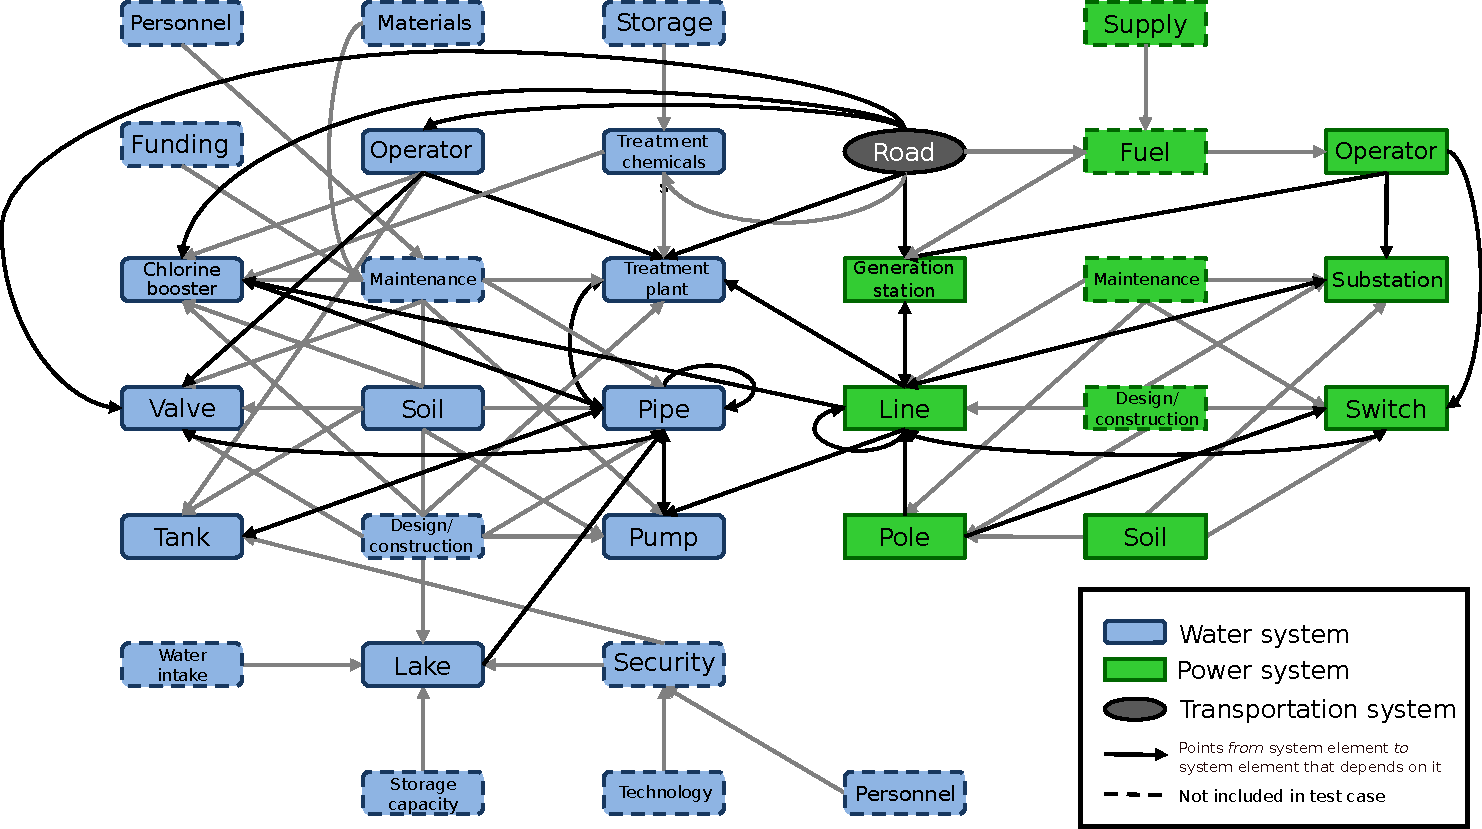
\includegraphics[width=20cm]{muirweb.pdf}}
\caption[Muir web for interdependent infrastructure system.]{\label{fig:ch4:muirweb}Muir web for interdependent infrastructure system consisting of water distribution, power distribution, and transportation systems. Dependencies between system elements are represented by arrows pointing \textit{from} a given system element \textit{to} an element which depends on it; for example, an arrow points from line to treatment plant, because the treatment plant requires power lines to supply electricity. Dashed lines represent elements not explicitly considered in our case study.}
\end{figure}

\vspace*{\fill}

\end{landscape}

%--------------------------------------------

%--------------------------------------------
% FIGURE ------------------------------------

\begin{landscape}

\vspace*{\fill}

\begin{figure}[!htp]
\centerline{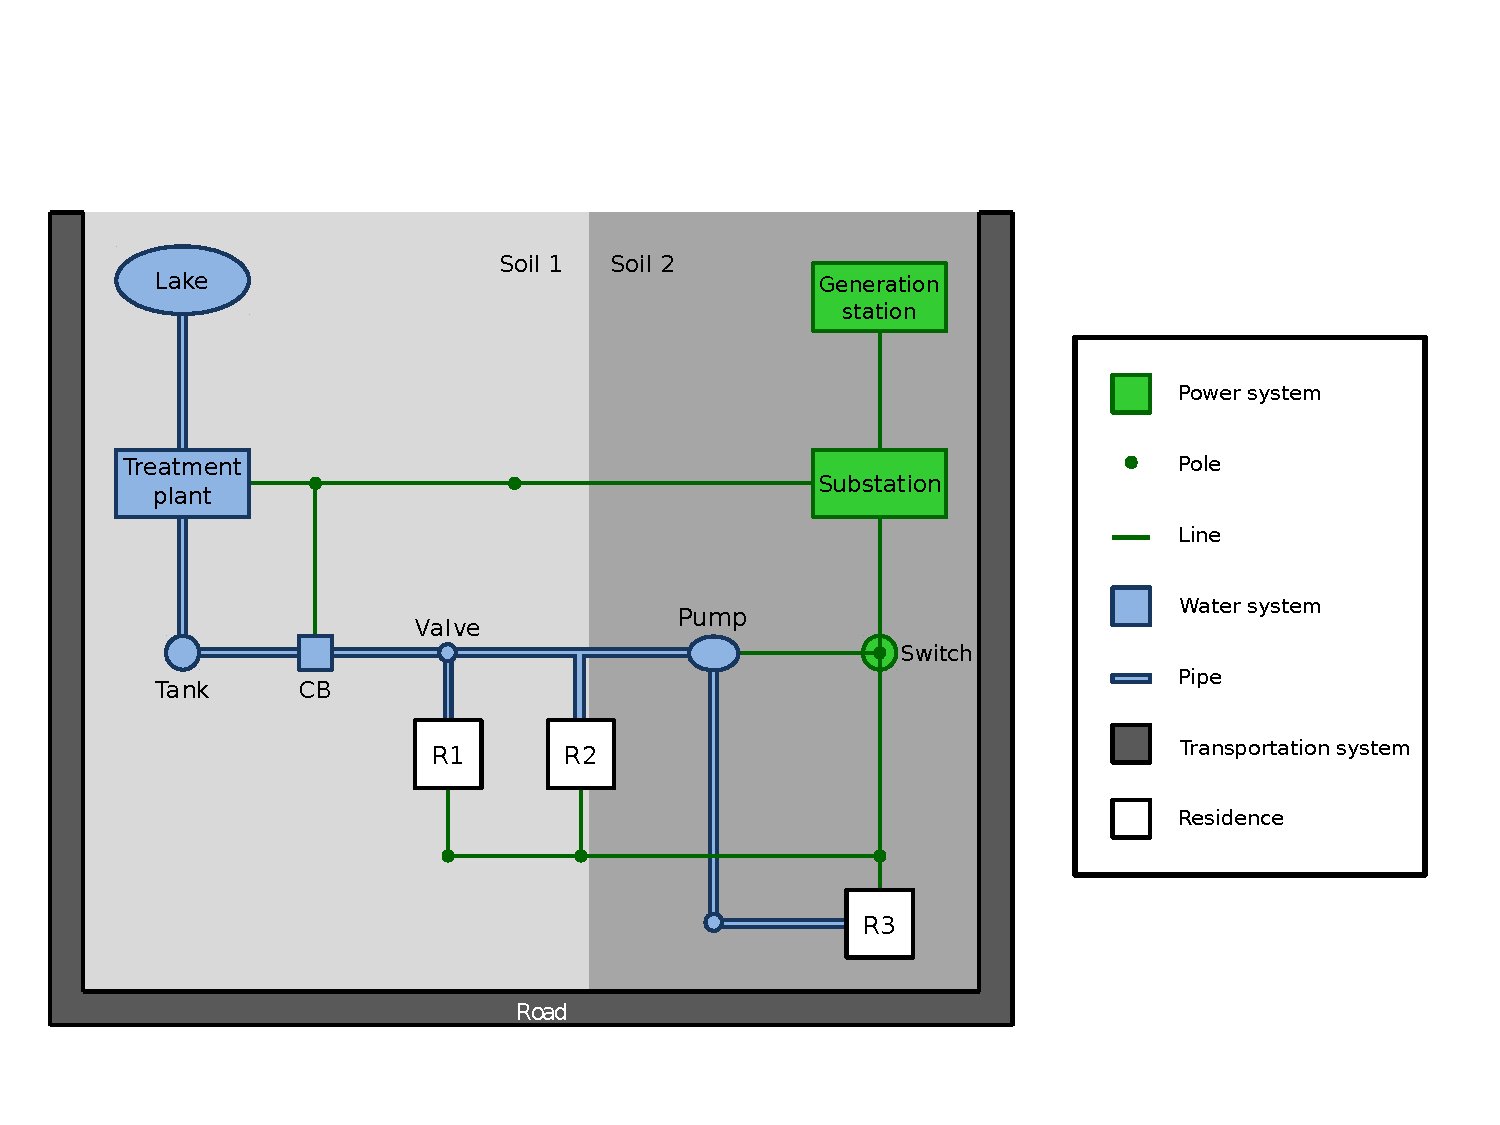
\includegraphics[trim=10 10 20 100,clip,width=20cm]{muirwebsystem.pdf}}
\caption[Fictitious infrastructure system used in simulations.]{\label{fig:ch4:infrastructures}Fictitious infrastructure system used in simulations.  Solid green lines represent power lines; solid green circles represent power poles; hollow blue lines represent water pipes. R1, R2, and R3 are residences.}
\end{figure}

\vspace*{\fill}

\end{landscape}

%--------------------------------------------

%--------------------------------------------
% TABLE -------------------------------------
\begin{table}
\small
\begin{center}
\begin{tabular}{lllll}

\toprule
\multirow{3}{*}{\textbf{Wind speed}} & \multirow{3}{*}{\textbf{Infrastructure}} & \multirow{3}{*}{\textbf{Residence}} & \textbf{P(failure)} & \textbf{P(failure)}\\
&&&\textbf{with inter-system}&\textbf{no inter-system}\\
&&&\textbf{dependencies}&\textbf{dependencies}\\

\midrule
75&Power&1&0.93&0.90\\
75&Power&2&0.87&0.80\\
75&Power&3&0.76&0.63\\
75&Water&1&0.98&0.85\\
75&Water&2&0.98&0.86\\
75&Water&3&1.00&0.95\\
75&Transportation&1&0.34&0.34\\
75&Transportation&2&0.34&0.34\\
75&Transportation&3&0.34&0.34\\
110&Power&1&1.00&1.00\\
110&Power&2&1.00&1.00\\
110&Power&3&1.00&0.99\\
110&Water&1&1.00&1.00\\
110&Water&2&1.00&1.00\\
110&Water&3&1.00&1.00\\
110&Transportation&1&0.72&0.72\\
110&Transportation&2&0.72&0.72\\
110&Transportation&3&0.72&0.72\\
\bottomrule
\end{tabular}
\end{center}

\caption{\label{tab:ch4:pfail}Probabilities of failure of power, water, and transportations at residences based on simulations.}

\end{table}
%--------------------------------------------

The simulation results are quantified as probabilities that power, water, or transportation will fail at each of the residences in our system when subjected to a hurricane; these results are summarized in Table \ref{tab:ch4:pfail}.  For both hurricane strengths, Residence 1 is most likely to lose power (P = 0.93 and 1.00 for 75 and 110 mph storms, respectively), followed by Residence 2 (P = 0.87 and 1.00 for 75 and 110 mph storms, respectively) and then Residence 3 (P = 0.76 and 1.00 for 75 and 110 mph storms, respectively).  These results correspond with the physical system as expected  --  Residence 1 is the furthest from the generation station with respect to network elements.  The opposite results are true for water; during a 75 mph storm, Residence 3 is most likely to lose water (P = 0.98), followed by Residence 2 (P = 0.98) and then Residence 1 (P = 1.00), again corresponding to distance from the source.  The simulation indicates that all residences will lose water during a 110 mph storm, a result of the dependency of the water system on the power and transportation systems, both of which have a high probability of failure during such a storm.

The results obtained from the simulations that included only intra-system dependencies (\emph{i.e.}, no dependencies between different infrastructure types) indicate lower probabilities of failure for both power and water at all residences than the simulations that included inter-system dependencies, described above.  Because the transportation system did not initially depend on either the power or the water system, the failure probabilities for each of the residences remain the same.  In particular, the probabilities of a residence losing water (P = 0.85, 0.86, and 0.95 for Residences 1, 2, and 3, respectively) and power (P = 0.89, 0.80, and 0.64 for Residences 1, 2, and 3, respectively) are markedly lower for a 75 mph storm than described above; this is likely in large part a result of the treatment plant’s dependence on both electric lines for power and roads for transportation of operators and chemicals and the generation station’s dependence on roads for operator transportation.  When these dependencies are not considered, failure probabilities are likely to be underestimated.  These results confirm the importance of considering dependencies between infrastructure systems, as well as other factors, such as the necessity of operators, as allowed by our Muir web approach.

%%%%%%%%%%%%%%%%%%%%%%%%%%%%%%%%%%%%%%%%%%%%%%%%%%%%%%%%%%%%%%%%%%%%%%%%%%%%%%%%%%%%%%%%%%

\section{Discussion}
\label{sec:ch4:discussion}

Muir webs provide a convenient model construct for expanding the factors considered in modeling the performance and reliability of interdependent infrastructure systems. While my approach still uses fragility curves, the use of a Muir web allows the types of dependencies included to be substantially expanded to incorporate both abiotic factors independent of the hazard load (\emph{e.g.}, soil type and it’s effect on foundation stability) and management factors (\emph{e.g.}, the availability of operators). This offers a significant advantage over existing approaches that assume both (1) the fragility curve is dependent on only a single demand parameter and (2) the failure events are conditionally independent given the value of the single underlying demand parameter. The Muir web approach provides the basis for a more realistic representation and estimation of the performance and reliability of interdependent infrastructure systems.

However, the increased flexibility and accuracy in the representation of the Muir web comes at a cost; more information is needed. A traditional fragility-based approach requires only the assignment of fragility curves that depend on single demand parameters. These curves exist for many elements of infrastructure systems for major hazards such as earthquakes and hurricanes. Muir webs, on the other hand, require a more complete accounting and consideration of the other factors that influence the performance of the elements of infrastructure systems. Each element must be examined individually, and those things that it depends on to function must be determined and included in the model, which is a challenging task. Yet without considering these additional factors, the resulting model is a significant approximation of reality.

%%%%%%%%%%%%%%%%%%%%%%%%%%%%%%%%%%%%%%%%%%%%%%%%%%%%%%%%%%%%%%%%%%%%%%%%%%%%%%%%%%%%%%%%%%%%%%%%%%%%%%%%%%%%%%%%%%%%%%%%